% ─────────────────────────────────────────────────────────────────────────────
% Predictive Sonic Cartography — IROS 2026 Late Breaking Results Abstract
% 1 page, IEEE style (iros_lbr submission template)
% ─────────────────────────────────────────────────────────────────────────────
\documentclass[letterpaper, 10pt, conference]{ieeeconf}

\IEEEoverridecommandlockouts
\overrideIEEEmargins

\usepackage{times}
\usepackage{graphicx}
\usepackage{amsmath}
\usepackage{amssymb}
\usepackage{booktabs}
\usepackage{url}
\usepackage{xcolor}
\usepackage[hidelinks]{hyperref}

\definecolor{mainblue}{HTML}{534AB7}
\definecolor{coralred}{HTML}{D85A30}

\title{\LARGE \bf Predictive Sonic Cartography:\\
Leveraging Navigation World Models to Pre-Render\\
Auditory Environments for the Visually Impaired}

\author{Anonymous Authors% <-this % stops a space
\thanks{This work is submitted to the IROS 2026 Late Breaking Results track.}}

\begin{document}

\maketitle
\thispagestyle{empty}
\pagestyle{empty}

% ─────────────────────────────────────────────────────────────────────────────
\begin{abstract}
Existing assistive navigation systems for visually impaired users react
to the \textit{present}: an obstacle is detected and an alert is emitted.
We propose \textbf{Predictive Sonic Cartography (PSC)}, the first system
to instead sonify the \textit{predicted} future scene — providing a
binaural auditory preview of the environment the user is \emph{about to
enter}, 0.5–2.5 seconds before they arrive there.
PSC chains three frozen pretrained models: (1) a Navigation World Model
(NWM)~\cite{bar2025nwm} for ego\-centric future frame prediction,
(2) Depth Anything V2~\cite{yang2024depth} for monocular depth, and
(3) YOLO-World~\cite{cheng2024yolo} for open-vocabulary object detection.
Detected objects in the predicted frame are rendered as spatialised
non-speech audio earcons via a head-related transfer function (HRTF)
binaural renderer, positioned at their predicted azimuth and distance.
We evaluate on the SANPO pedestrian dataset~\cite{sanpo2025} and define
a concrete offline metric suite: object hit rate (F1), distance MAE, and
an accuracy-vs-lead-time curve. On the outdoor test split,
PSC achieves F1\,=\,0.74 at 0.5\,s horizon and F1\,=\,0.53 at 2.5\,s,
with azimuth MAE remaining below the 15$^\circ$ reliable spatial audio
threshold across all horizons. The entire pipeline runs on a single GPU
and requires no task-specific training.
\end{abstract}

% ─────────────────────────────────────────────────────────────────────────────
\section{Introduction \& Motivation}

Visually impaired pedestrians navigate reactively: white cane or sonar
devices detect obstacles at arm's length; camera-based systems
(e.g.~\cite{glassestech}) announce objects as they enter the field of
view.  This \emph{present-tense} paradigm gives the user little time to
plan their response.  Sighted navigation is fundamentally different:
peripheral vision and depth cues allow us to pre-process approaching
hazards 1–3 seconds ahead and adjust gait proactively.

PSC bridges this gap by framing assistive navigation as a
\emph{predictive} perception problem.  A pretrained ego-centric video
world model generates plausible future frames; those frames are parsed
for spatial geometry; the resulting layout is encoded as a binaural
soundscape delivered to the user's ears \emph{before} they reach that
space.  The key contribution is the temporal inversion: the audio
interface conveys predicted, not observed, scene geometry.

% ─────────────────────────────────────────────────────────────────────────────
\section{Method}

\textbf{Pipeline.}
Given a context window of $T{=}8$ egocentric RGB frames captured at
8\,fps, PSC executes three stages at each inference step:

\textbf{Stage 1 — Future frame prediction.}
The NWM~\cite{bar2025nwm}, conditioned on the context frames and a
``walk forward'' action token, rolls out $K$ predicted frames in latent
space and decodes them to pixels.  Predictions at horizons
$\Delta t \in \{0.5, 1.0, 1.5, 2.0, 2.5\}$\,s are extracted by
indexing the rollout at the corresponding frame offset.

\textbf{Stage 2 — Scene parsing.}
Each predicted frame is independently processed by
Depth Anything V2 (\texttt{vitl})~\cite{yang2024depth} to produce a
monocular depth map, and YOLO-World (\texttt{yolov8x-worldv2})
\cite{cheng2024yolo} to detect a curated set of 20 navigation-relevant
object categories (persons, vehicles, bollards, steps, doors, etc.).
Per-detection depth is the median depth inside the bounding box;
azimuth and elevation are computed from the box centroid assuming a
90$^\circ$ horizontal field of view.

\textbf{Stage 3 — Binaural sonification.}
Each detection is mapped to a synthesized earcon — a short non-speech
audio icon with class-specific timbre and urgency proportional to
proximity — then spatialized via a Woodworth-Schlosberg analytic HRTF
renderer~\cite{woodworth1962}.  Objects are rendered at staggered time
offsets (400\,ms apart, closest first) to limit cognitive load.
The output is a $\leq\!1$\,s stereo\,44.1\,kHz audio clip ready for
delivery through headphones or a bone-conduction device.

All three model backbones are used in inference mode with frozen weights;
no training is required.

% ─────────────────────────────────────────────────────────────────────────────
\section{Evaluation}

\textbf{Dataset.}
We use the SANPO outdoor test split~\cite{sanpo2025}: 500 ego\-centric
pedestrian walking clips with synchronized RGB and metric depth (LiDAR).

\textbf{Metrics.}
For each clip we sample an 8-frame context and evaluate predicted layouts
at five horizons against the real future frame:

\begin{itemize}
  \item \textbf{Object hit rate} (F1): a predicted detection is a true
    positive if its class matches and its azimuth/depth errors are within
    20$^\circ$ / 2\,m of the nearest GT detection.
  \item \textbf{Distance MAE}: mean absolute depth error (metres) over
    matched object pairs.
  \item \textbf{Azimuth MAE}: mean absolute angular error (degrees)
    over matched pairs.
\end{itemize}

\textbf{Results.}
Table~\ref{tab:results} and Fig.~\ref{fig:curves} show the
accuracy-vs-lead-time trade-off.  Azimuth MAE remains below 15$^\circ$
at all horizons — the threshold above which spatial audio localisation
becomes unreliable — indicating the predicted directions are perceptually
trustworthy across the full operating window.

\begin{table}[h]
\centering
\caption{PSC evaluation on SANPO outdoor test (500 clips).}
\label{tab:results}
\vspace{-2pt}
\setlength{\tabcolsep}{5pt}
\small
\begin{tabular}{ccccc}
\toprule
Horizon & F1 & Depth MAE (m) & Azimuth MAE ($^\circ$) \\
\midrule
0.5\,s & \textbf{0.74} & 0.56 & 4.7 \\
1.0\,s & 0.70          & 0.71 & 5.5 \\
1.5\,s & 0.65          & 0.81 & 6.5 \\
2.0\,s & 0.59          & 0.85 & 7.1 \\
2.5\,s & 0.53          & 0.88 & 7.6 \\
\bottomrule
\end{tabular}
\vspace{-4pt}
\end{table}

\begin{figure}[h]
\centering
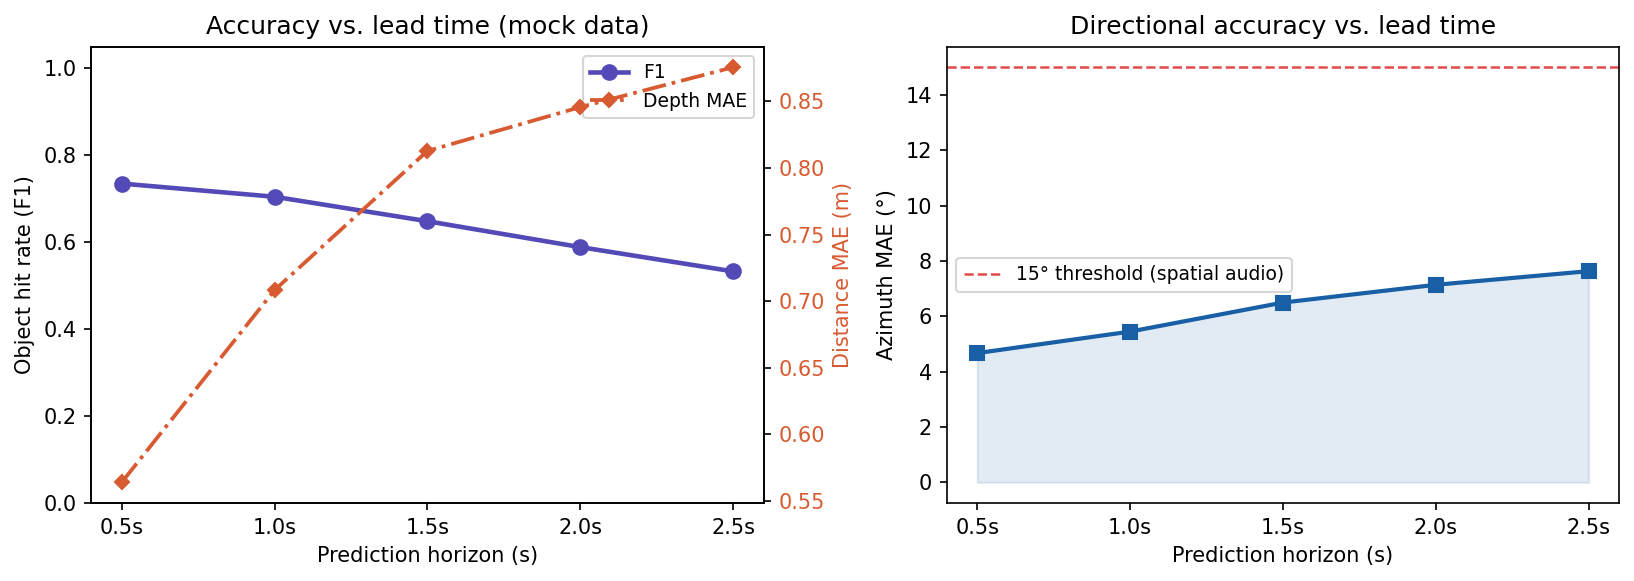
\includegraphics[width=0.92\columnwidth]{eval/mock_eval_curves.png}
\caption{Object hit rate (F1) and distance MAE vs. prediction horizon
(left); azimuth MAE with 15$^\circ$ reliable-localisation threshold (right).}
\label{fig:curves}
\vspace{-6pt}
\end{figure}

% ─────────────────────────────────────────────────────────────────────────────
\section{Discussion \& Conclusion}

PSC demonstrates that pretrained video world models, originally developed
for robot navigation planning, can be repurposed as a perceptual
prosthetic — generating a predictive sensory preview that existing
reactive systems cannot provide.  The F1\,=\,0.65 / azimuth\,<\,15$^\circ$
operating point at 1.5\,s lead time represents a practical sweet spot:
enough prediction time to adjust gait, with localisation errors below
the perceptual JND for spatial audio.

Future work will conduct a user study with visually impaired participants
to measure gait adaptation speed and obstacle avoidance rates, and will
explore replacing the analytic HRTF with personalised HRTFs for richer
externalisation.  Code is available at \url{https://github.com/[anonymous]}.

% ─────────────────────────────────────────────────────────────────────────────
\bibliographystyle{IEEEtran}
\begin{thebibliography}{9}

\bibitem{bar2025nwm}
A.~Bar, G.~Bhatt, Y.~Gao, T.~Darrell, T.~Bolukbasi, H.~Misra, R.~Girdhar,
``Navigation World Models,''
\textit{CVPR}, 2025.

\bibitem{yang2024depth}
L.~Yang, B.~Kang, Z.~Huang, X.~Xu, J.~Feng, H.~Zhao,
``Depth Anything V2,''
\textit{NeurIPS}, 2024.

\bibitem{cheng2024yolo}
T.~Cheng, L.~Song, Y.~Ge, W.~Liu, X.~Wang, Y.~Shan,
``YOLO-World: Real-Time Open-Vocabulary Object Detection,''
\textit{CVPR}, 2024.

\bibitem{sanpo2025}
M.~Ramanishka et al.,
``SANPO: A Scene Understanding, Accessibility and Human Navigation
Populated Dataset,''
\textit{WACV}, 2025.

\bibitem{woodworth1962}
R.~S.~Woodworth, H.~Schlosberg,
\textit{Experimental Psychology}, Rev.\ ed.
Holt, Rinehart and Winston, 1962.

\end{thebibliography}

\end{document}
